\documentclass[border=10pt]{standalone}
\usepackage{tikz,amsmath}
\usetikzlibrary{arrows.meta}

% ========== 配色 ==========
\definecolor{inFill}{RGB}{183,224,177}
\definecolor{inLine}{RGB}{32,102,32}
\definecolor{hidFill}{RGB}{199,203,243}
\definecolor{hidLine}{RGB}{52,58,143}
\definecolor{orFill}{RGB}{250,224,180}
\definecolor{orLine}{RGB}{190,110,20}
\definecolor{outFill}{RGB}{243,199,199}
\definecolor{outLine}{RGB}{143,52,52}
\definecolor{blFill}{RGB}{214,228,250}
\definecolor{blLine}{RGB}{60,90,170}

\begin{document}
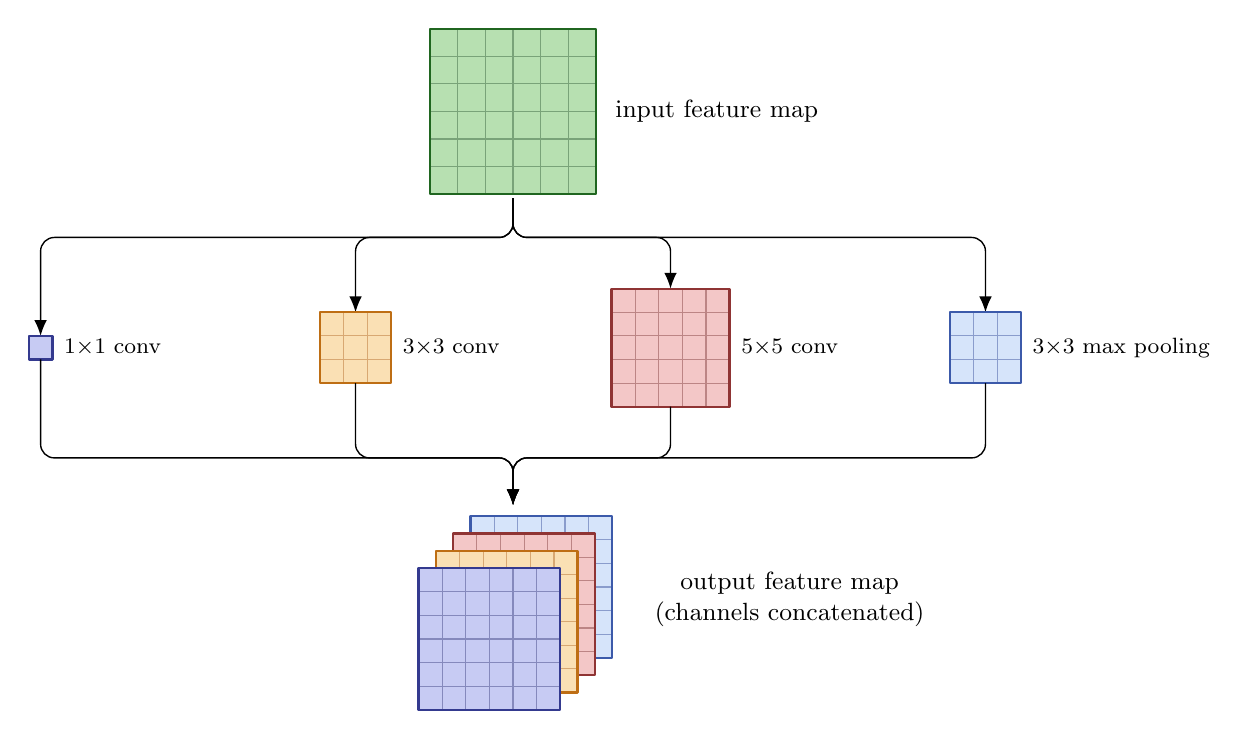
\begin{tikzpicture}[
    font=\small, line join=round,
    every node/.style={inner sep=0pt, outer sep=0pt},
    >={Latex[length=2mm, width=1.6mm]},
    arr/.style={->, line width=.5pt, rounded corners=5pt}
  ]

  % ========== 网格方块宏 ==========
  \newcommand{\gridbox}[5]{%
    \fill[#5Fill] (#1,#2) rectangle (#1+#3*#4, #2+#3*#4);
    \draw[step=#4, #5Line!60, line width=.4pt, shift={(#1,#2)}] (0,0) grid (#3*#4, #3*#4);
    \draw[#5Line, thick] (#1,#2) rectangle (#1+#3*#4, #2+#3*#4);
  }

  % ========== 顶部：输入特征图 ==========
  \gridbox{-1.05}{5.15}{6}{.35}{in}
  \node[anchor=west] at (1.3,6.2) {input feature map};

  % ========== 输入 -> 四分支（箭头接到各盒顶边） ==========
  \draw[arr] (0,5.1) -- (0,4.6) -- (-6,4.6) -- (-6,3.35);
  \draw[arr] (0,5.1) -- (0,4.6) -- (-2,4.6) -- (-2,3.65);
  \draw[arr] (0,5.1) -- (0,4.6) -- (2,4.6)  -- (2,3.95);
  \draw[arr] (0,5.1) -- (0,4.6) -- (6,4.6)  -- (6,3.65);

  % ========== 四分支：格子数 = 核/窗口尺寸（1 / 3x3 / 5x5 / 3x3），垂直居中 y=3.2 ==========
  \gridbox{-6.15}{3.05}{1}{.3}{hid}
  \node[anchor=west, font=\footnotesize] at (-5.7,3.2) {1$\times$1 conv};

  \gridbox{-2.45}{2.75}{3}{.3}{or}
  \node[anchor=west, font=\footnotesize] at (-1.4,3.2) {3$\times$3 conv};

  \gridbox{1.25}{2.45}{5}{.3}{out}
  \node[anchor=west, font=\footnotesize] at (2.9,3.2) {5$\times$5 conv};

  \gridbox{5.55}{2.75}{3}{.3}{bl}
  \node[anchor=west, font=\footnotesize] at (6.6,3.2) {3$\times$3 max pooling};

  % ========== 四分支 -> 汇合 -> 拼接堆（从各盒底边出发） ==========
  \draw[arr] (-6,3.05) -- (-6,1.8) -- (0,1.8) -- (0,1.2);
  \draw[arr] (-2,2.75) -- (-2,1.8) -- (0,1.8) -- (0,1.2);
  \draw[arr] (2,2.45)  -- (2,1.8)  -- (0,1.8) -- (0,1.2);
  \draw[arr] (6,2.75)  -- (6,1.8)  -- (0,1.8) -- (0,1.2);

  % ========== 底部：通道维拼接 ==========
  \gridbox{-0.54}{-0.74}{6}{.3}{bl}
  \gridbox{-0.76}{-0.96}{6}{.3}{out}
  \gridbox{-0.98}{-1.18}{6}{.3}{or}
  \gridbox{-1.2}{-1.4}{6}{.3}{hid}
  \node[anchor=west, align=center] at (1.8,0)
    {output feature map\\(channels concatenated)};

\end{tikzpicture}
\end{document}